\section{Schema concettuale}

\begin{figure}[h!]
	\centering
	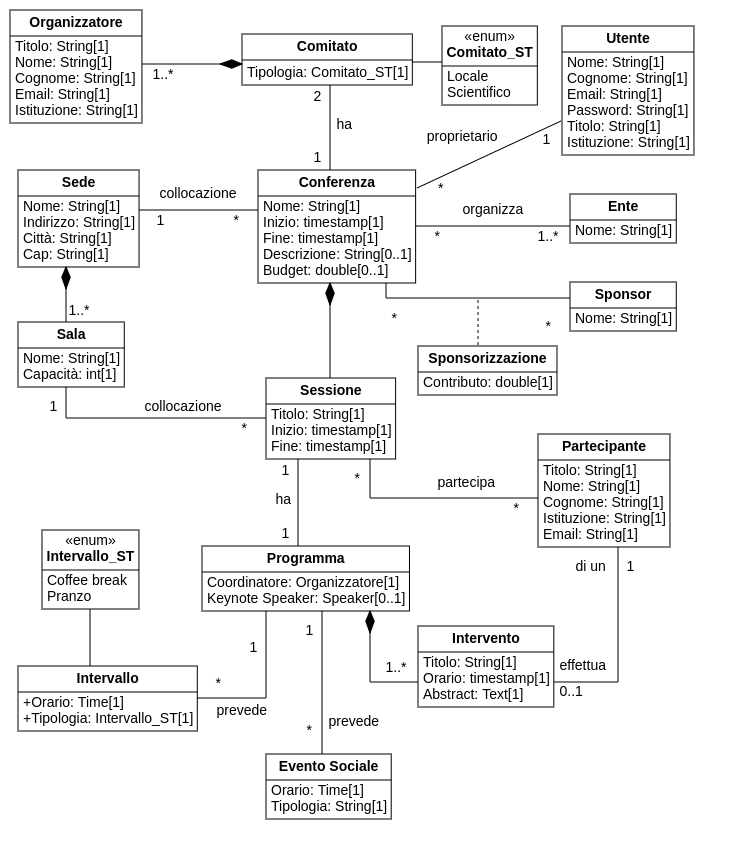
\includegraphics[scale=0.6]{Immagini/Schema_Concettuale.png}
	\caption{Schema concettuale del problema}\label{uml:schema_concettuale}
\end{figure}
Nella Figura \ref{uml:schema_concettuale} è presente lo schema concettuale della base di dati descritta nella sezione \ref{sez:traccia}.

\section{Ristrutturazione dello schema concettuale}

\subsection{Rimozione degli attributi multivalore}All'interno del diagramma delle classi mostrato in Figura \ref{uml:schema_concettuale} sono presenti vari attributi multivalore. Per ciascuno di essi sono state fatte le seguenti valutazioni:
\begin{enumerate}
	\item Si partiziona l'attributo \textit{Indirizzo} presente in \textsc{Sede} suddividendolo in vari campi \textit{Via}, \textit{Civico}, \textit{Cap}, \textit{City}, \textit{Provincia} e \textit{Nazione} e creando una nuova entità chiamata \textsc{Indirizzo}.
	\item Si è deciso di partizionare l'attributo \textit{Valuta} presente nella classe di associazione \textsc{Sponsorizzazione} creando una nuova classe chiamata \textsc{Valuta}.
\end{enumerate}
\subsection{Rimozione classi di associazione}
All'interno dello schema concettuale è presente la classe di associazione \textsc{Sponsorizzazione} all'interno dell'associazione [*...*] tra \textsc{Conferenza} e \textsc{Sponsor}. Nello schema ristrutturato questa è stata rimossa reificandola e scindendo l'associazione in due associazioni di tipo [1..*].
\subsection{Rimozione generalizzazioni}
Per quanto riguarda la rimozione delle generalizzazioni presenti nello schema concetuale:
\begin{enumerate}
	\item Nel caso delle entità \textsc{Comitato Scientifico} e \textsc{Comitato Locale} che specializzano la classe \textsc{Comitato} si è optato per l'accorpamento delle classi figlie all'interno della superclasse attraverso la specifica di una enumerazione chiamata \textsc{Comitato\_ST} composta dai campi \textit{Scientifico} e \textit{Locale};
	\item Nel caso delle entità \textsc{Pranzo} e \textsc{Coffee Break} che specializzano la classe \textsc{Intervallo} si è adottato la stessa politica.
\end{enumerate}
\subsection{Scelta degli identificatori principali}
Risulta conveniente ai fini di una migliore traduzione delle associazioni l’introduzione di chiavi
surrogate per ogni entità. Tali chiavi altro non saranno che identificativi numerici interi del tipo \textit{Id\_NomeEntità}, eccezion fatta per l'entità \textsc{Valuta} la quale viene identificata univocamente da una stringa di tre caratteri stando allo standard ISO 4217\footnote{ISO 4217 è uno standard internazionale che descrive codici di tre lettere per definire i nomi delle valute, stabilito dall'Organizzazione internazionale per la normazione (ISO), che viene usato comunemente nel sistema bancario e nel mondo economico, nonché nella stampa specializzata.}.
\begin{figure}[h!]
	\centering
	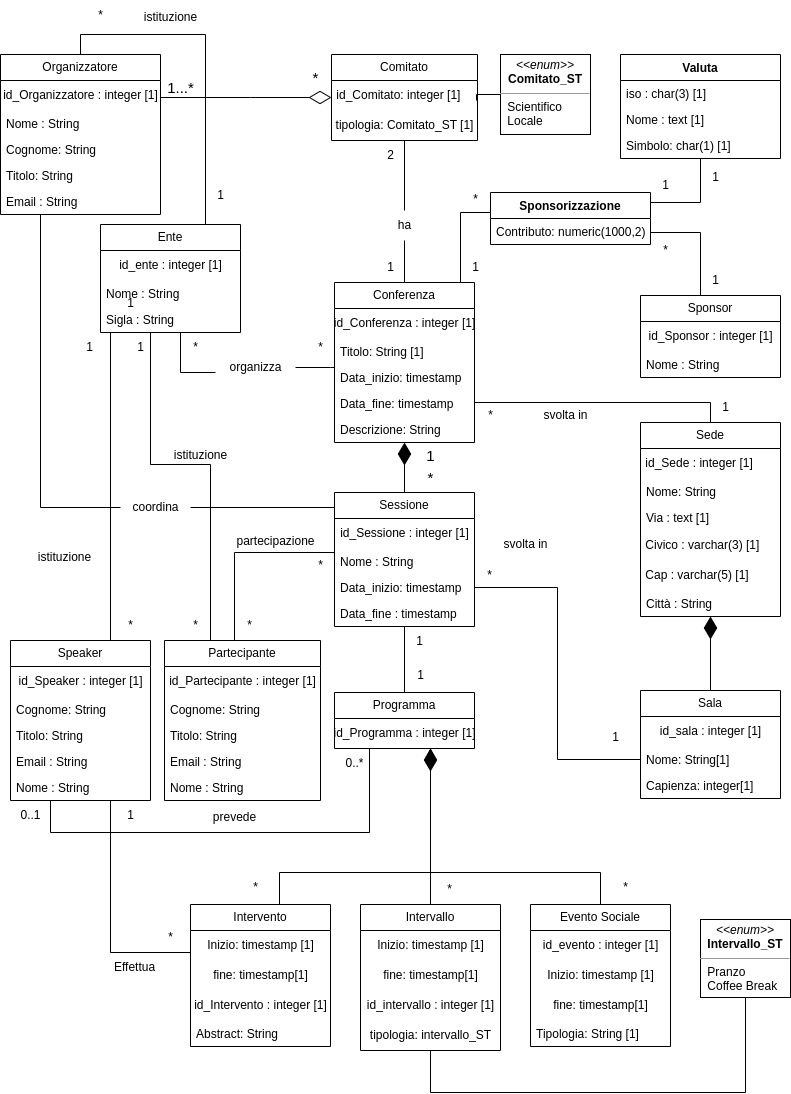
\includegraphics[scale=0.55]{Immagini/Ristrutturato_finale.png}
	\caption{Ristrutturazione dello schema concettuale}\label{uml:schema_ristrutturato}
\end{figure}